\documentclass[a4paper]{article}

\usepackage[a4paper, top=2in, bottom=1.5in, left=1in, right=1in]{geometry}
\usepackage{amsmath}
\usepackage{amssymb}
\usepackage{graphicx}
\usepackage{float}

\usepackage{fontspec}
\setmainfont{Open Sans Light}
\setmonofont[Scale=0.9]{Source Code Pro Light}

\setlength{\parindent}{0cm}

\begin{document}

\title{\textbf{IT and Values \\ Lectures}}
\author{\texttt{https://github.com/hylkev/ethiek-en-recht-bullet-points}}
\date{April, 2014}
\maketitle

\section{First Lecture : Intro into Ethics}

\begin{description}
\item[Ethics] is that branch of philosophy investigating issues of "the good"
\item[Metaethics] is the attempt to judge ethical theories
\item[Normative ethics] attempts to derive standards of rightness or wrongness
\end{description}

\subsection*{Virtue Ethics}

\begin{description}
\item[Plato : cardinal virtues:] wisdom, courage, temperance, justice
\item[Other virtues:] fortitude, generosity, self-respect, good temper, sincerity
\item[Vices:] cowardice, insensibility, injustice, vanity
\item[Aristotle:] virtues are means between extreme character traits (excess/mean/deficiency)
\item[Thomas Aquinas : Christian virtues:] faith, hope, charity
\end{description}

\subsection*{Deontology (From Greek: δέον = duty)}

\begin{description}
\item[Duty theories] base morality on specific, foundational principles of duty
\item[Samuel Pufendorf] classified duties under three headings:
\begin{itemize}
\item Duties to God
\begin{itemize}
\item know the existence and nature of God
\item worship God
\end{itemize}
\item Duties to Oneself
\begin{itemize}
\item duties of the soul (skills, talents, ...)
\item duties to the body
\end{itemize}
\item Duties to Others
\begin{itemize}
\item Absolute duties (avoid wronging, treat as equals, promote the good)
\item Conditional duties (contracts between people)
\end{itemize}
\end{itemize}
\item[John Locke: rights theory:] The laws of nature mandate that we should not harm anyone's life, health, liberty or possessions
\item[Natural rights] are
\begin{description}
\item[Natural:] not invented or created by governments
\item[Universal:] do not change from country to country
\item[Equal:] same for all people, regardless of gender, race or handicap
\item[Inalienable:] one cannot hand over rights to another person
\end{description}
\item[Immanuel Kant: categorical imperative:] mandates an action, \textit{regardless of desires}
\item[``Treat people as an end,] \textbf{and never as a means to an end''}
\item[``Act only according to that maxim] \textbf{by which you can at the same time will that it would become a universal law''}
\end{description}

\subsection*{Consequentialism}

\begin{description}
\item[Good conduct] is determined solely by a cost-benefit analysis of an action's consequences.
\item[Teleological] theories
\begin{description}
\item[Ethical Egoism:] consequences are more favourable to me
\item[Ethical Altruism:] consequences are more favourable to everyone except me
\item[Utilitarianism:] consequences increase overall happiness
\end{description}
\item[Hedonistic utilitarianism:] pleasure and pain are the only consequences that matter
\item[Jeremy Bentham : act-utilitarianism:] tally the consequences of each action we perform
\item[John Stuart Mill:] place certain pleasures above others \\ intellectual pleasures $>$ bodily pleasures
\item[Rule-utilitarianism:] morality of adoption of rules
\end{description}

\section{Second Lecture : Cybercrime}

\textbf{Some criminal acts are facilitated by ICT. Others are only possible because the technology exists.}

\begin{description}
\item[Crime:] some act + intentional state made explicitly forbidden by law
\item[Kevin Mitnick: ] Hacking
\item[Fraud:] wrongful or criminal deception intended to result in financial or personal gain.
\item[Computer Fraud:] dishonest misrepresentation, let another do or refrain from doing something which causes loss.
\begin{itemize}
\item Altering, destroying, suppressing or stealing output
\item Altering or deleting stored data
\item Altering or misusing existing system tools or software packages
\item Altering or writing code for fraudulent purposes
\end{itemize}
\item[Espionage:] Markus Hess / Lawrence Berkley Laboratories
\item[Espionage or spying] involves a government or individual obtaining information considered secret or confidential without the permission of the holder of the information
\item[Speech / Expression] involves
\begin{description}
\item[Obscenity:] Child pornography, locally obscene materials
\item[Harassment:] Directed at specific individuals or groups
\item[Threats:] intimidation with implication of harm
\end{description}
\end{description}

\subsection*{Property}

\begin{description}
\item[Goods:] Theft
\item[Ideas:] Intellectual Property
\end{description}

\subsection*{Cyber Terrorism / Other}

Anonymous, Kim Dotcom, Edward Snowden, Silk Road, Bitcoin

\section{Third Lecture : Value Sensitive Design}

\begin{description}
\item[Empirical Research] forms the middle ground between \textbf{Subjective} and \textbf{Objective} theories
\item[Prudential-Empirical Ethics of Technology]~
\begin{itemize}
\item empirical findings that \textit{suggest} what kinds of experiences and activities \textit{tend to} increase subjective well-being
\item critical evaluation of validity and causal relationships
\item translate into concrete technological features
\item minimise negative side-effects
\end{itemize}
\item[Ed Diener's Satisfaction With Life Scale (SWLS)] measures life-satisfaction
\begin{itemize}
\item Overall life satisfaction
\item Real-time pings
\end{itemize}
\item[Positive Psychology:] The scientific study of what constitutes subjective well-being and how it can be enhanced
\item[Flow] Transformation of time
\begin{figure}[H]
\centering
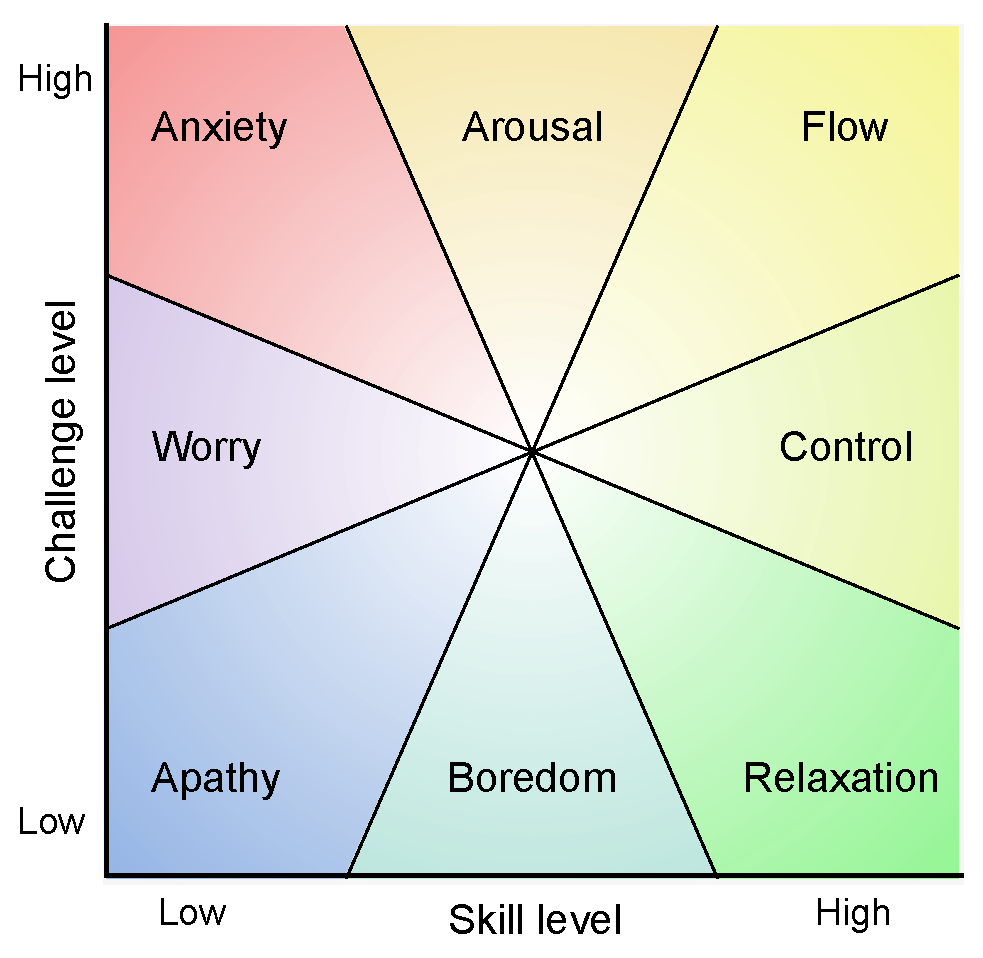
\includegraphics[width=0.4\textwidth]{pictures/Flow}
\caption{Flow}
\end{figure}
\item[Absolute wealth vs relative wealth] ~
\item[Being social and belonging to a community] is a strong determinant
\item[Sensory pleasure] is strongest when the brain accomplishes a difficult task unexpectedly
\item[User Interface] must allow for users at cognitive and autonomous stages
\item[The ideal user interface] continuously co-adapts to user in such a way that an expert's usage will in practice be incomprehensible to novice
\item[Online altruism] can be entirely illusory, giving well-being benefit without actually doing anything good for the world (\textbf{Slacktivism})
\end{description}

\section{Fourth Lecture : Privacy and ICT}

\begin{description}
\item[Privacy] is the right to be left alone
\item[Privacy] is the right to control what others know about you
\item[Forms of privacy:] ~
\begin{itemize}
\item Personal
\item Territorial
\item Communications
\item Informational
\end{itemize}
\item[Openness and transparency:] there should be no secret record keeping
\item[Individual participation:] the subject of a record should be able to see and correct the record
\item[Collection limitation:] data collection should be proportional
\item[Data quality:] data should be relevant to the purpose
\item[Use limitation:] Data should only be used for their specific purpose by authorized personnel
\item[Reasonable security:] Adequate security safeguards
\item[Accountability:] Record keepers must be accountable for compliance with these principles
\item[Convenience:] free flow of information $\leftrightarrow$ personal risks
\item[Communitarian:] give up privacy for the greater good
\item[Egalitarian:] everybody has access to the same information ``transparent society''
\item[Hoffman] (1980):
\begin{itemize}
\item the right to determine what information to share
\item the right to know what is being collected
\item the right to access data
\end{itemize}
\item[Westin] classes people into three distinct groups:
\begin{itemize}
\item fundamentalists alsways choose privacy
\item unconcerned individuals are willing to forego most privacy claims in exchange for service benefits
\item pragmatists weigh the benefits of services against the degree of personal information sought
\end{itemize}
\end{description}

\section{Fifth Lecture}
\section{Sixth Lecture : Democracy and ICT}

The nature of the medium of ICT is inherently linked to maximal freedom.

Ideas vs artifacts

"Expression"

Copyright vs Patent



\section{Seventh Lecture}

%\begin{itemize}
%\item 
%\end{itemize}

%\begin{description}
%\item[]
%\end{description}

\end{document}